
\documentclass[conference]{IEEEtran}
\usepackage {graphicx} 
\usepackage{algorithm2e}
\RestyleAlgo{ruled}
\usepackage{algpseudocode}


% Judul
\title{Implementasi Algoritmass Dijkstra}

% Author
\author{\IEEEauthorblockN{Rani Isramiharti}
\IEEEauthorblockA{\textit{School of Electrical Engineering and Informatics}\\
\textit{Institut Teknologi Bandung}\\
Bandung, Indonesia\\
email: 13220003@std.stei.itb.ac.id}
}

\begin{document}
\maketitle
\begin{abstract}
Kebun Raya Purwodadi dengan luas area sekitar 85 hektar ternyata kekurangan papan informasi yang menyebabkan pengunjung kerap kali kebingungan dalam mencari lokasi tanaman tertentu. Paper ini bertujuan untuk membuat simulasi dari algoritma yang dapat menentukan jarak terdekat antara pengunjung (pengguna program) dengan lokasi tanaman yang dituju. Algoritma yang digunakan adalah algoritma Dijkstra yang beroperasi secara menyeluruh (greedy) untuk menguji seitap persimpangan (Vertex) dan jalan (Edge) pada Kebun Raya Purwodadi. Berdasarkan hasil simulasi dan pengujian, kompleksitas ruang dari program ini adalah O(V) karena adanya pembentukan array yang berisi V nodes untuk mencari heap min imum. Sementara, kompleksitas waktu dari algoritma tersebut adalah O($\textbf V^\textbf2$ ).
\end{abstract}

\begin{IEEEkeywords}
Dijkstra, Vertex, Edge, Tanaman
\end{IEEEkeywords}

\section{Introduction}
	Studi mengenai penggunaan algoritma Dijkstra dalam mencari jarak terdekat dapat diimplementasikan pada kasus pencarian tanaman pada Kebun Raya Purwodadi seperti yang telah dilakukan oleh Yusuf et al di tahun 2017\cite{yusuf2017implementasi} . Paper ini bertujuan untuk melakukan simulasi kembali terhadap penelitian yang telah dilakukan dengan bahasa C serta mengevaluasi efisiensinya melalui perhitungan kompleksitas waktu dan ruang dengan analisis Big-O.

	Di Kecamatan Purwodadi, Kabupaten Pasuruan, terdapat salah satu kebun raya di Indonesia yang bernama Kebun Raya Purwodadi yang memiliki luas area hingga 85 hektar. Kebun raya sebagai fasilitas rekreasi dan penelitian ini ternyata kekurangan papan informasi yang seharusnya disediakan oleh pihak pengelola. Hal ini menyebabkan banyaknya pengunjung yang merasa kebingungan untuk mencari lokasi dari tanaman tertentu. Oleh karena itu, Yusuf et al (2017) memutuskan untuk membuat suatu aplikasi dengan memanfaatkan algoritma Dijkstra untuk membantu pengunjung Kebun Raya Purwodadi dalam mencari lokasi tertentu.

	Algoritma Dijkstra digunakan karena algoritma ini dapat beroperasi secara menyeluruh (algoritma greedy) terhadap semua alternatif fungsi serta durasi eksekusi yang lebih cepat jika dibandingkan dengan algoritma serupa, yaitu Bellman-Ford. Algoritma ini akan mencari jalur dengan ’biaya’ atau cost terendah antara dua titik dengan membandingkan semua alternatif yang ada.

	Pada kasus ini, masing-masing persimpangan di Kebun Raya Purwodadi direpresentasikan sebagai vertex dan setiap jalan direpresentasikan sebagai edge. Rute terdekat yang didapatkan akan diperoleh dari pembobotan setiap vertex dan edge berdasarkan jarak antara titik pengguna dengan titik tujuan atau tanaman.

\section{Studi Pustaka}
\subsection{Algoritma Dijkstra}

\begin{algorithm}
\caption{Dijkstra's Algorithm \ttfamily{Dijkstra}}\label{alg:one}
\KwResult{Find the shortest path from a to z}
\textbf{procedure} \textit{Djikstra}(G : weighted connected simple graph, with all weights positive)
\newline
\{\textit G has vertices $a = v_0,v_1, ..., v_n = z$ and lenghts $w(v_i, v_j)$ where $w(v_i, v_j) = \infty$ if $v_i, v_j$ is not an edge in \textit G\}
\newline
\For{i:= 1 \emph{\KwTo} n}{
	$L(v_i) := \infty$
	}
$L(a) := 0 $
\newline
$S := \emptyset$ 

\{the labels are now initialized so that the label of $a$ is 0 and all other labels are$\infty$, and $S$ is the empty set\}
\While{$z \epsilon S$}{
	\For{all verticles v not in S}{
		\If{L(u) + w(u, v) < L(v)}{
			$L(v) := L(u) + w(u, v)$
			\newline
			\{this adds a vertex to $S$ with minimal label and updates the labels of vertices not in S\}
}
}
}
\Return{L(z) = length of a shortest path from a to z}
\end{algorithm}

	Algoritma Dijkstra adalah algoritma yang digunakan untuk menemukan jarak jalur terpendek antara dua vertice pada graph berbobot dan tidak berarah sederhana\cite{rosen2012discrete}. Berbobot berarti grafik memiliki edge dengan suatu ’bobot’ atau harga. Bobot dapat merepresentasikan jarak, waktu, atau apapun yang memodelkan koneksi antara kedua node. Tidak berarah memiliki arti bahwa untuk setiap node yang terhubung, kita dapat mendekati suatu node dari kedua arah. Pendekatan Di jikstra juga memiliki asumsi bahwa bobot pada edge memiliki nilai yang tidak negatif. Hal ini karena nilai bobot akan terus dibandingkan dan diambil nilai yang paling kecil. Ada banyak varian pada algoritma ini, namun pada percobaan ini digunakan varian dimana suatu node ditetapkan menjadi source node. Dari node inilah akan dicari jarak terpendek diantara node lain. Algoritma ini dicetuskan oleh Edsger Wybe Dijkstra, salah seorang tokoh ternama di bidang computer science\cite{dijkstra1959note}. Kompleksitas dari algoritma dijkstra adalah O($n^2$), dengan n menyatakan jumlah vertice dari graph yang bersangkutan.
\subsection{Kebun Raya Puwodadi}
	Kebun Raya Purwodadi adalah kebun penelitian di Kecamatan Purwodadi, Jawa Timur. Ia juga dikenal dengan nama Hortus Ilkim Kering Purwodadi dan didirikan tanggal 30 Januari 1941 oleh Dr. L.G.M. Baas Becking. Sebagai cabang dari Kebun Raya Bogor, ia memiliki fungsi mengkoleksi tumbuhan yang hidup di dataran rendah kering. Sebagai Balai Konservasi Tumbuhan di bawah Pusat Konservasi Tumbuhan Kebun Raya, Kedeputian Bidang Ilmu Pengetahuan Hayati LIPI, kebun raya ini memiliki banyak tumbuhan yang dinaunginya. Dengan menggunakan algoritma Dijkstra, diharapkan ia dapat membantu pengunjung mencari tanaman tertentu maupun jarak yang paling optimal.
\section{metodologi penelitian}
	Peneliti menggunakan beberapa tahap dalam penyusunan paper ini. Pertama, dilakukan pengkajian dan studi literatur dengan membaca referensi paper yang berkaitan dan memilih paper yang dapat menjadi acuan dalam penelitian yang dilakukan, sehingga dari pilihan topik dan tema yang berkaitan secara luas dapat dikecilkan menjadi sebuah paper yang mencakup mayoritas dari topik yang dibahas. Setelah ditemukan beberapa paper, dilakukan perangkuman untuk menentukan paper yang sesuai sekaligus membahas poin-poin penting dari paper yang ingin dicapai. Setelah kedua tahap tersebut dilewati, penentuan paper yang dijadikan prototype penelitian merupakan hal yang mudah dan menjadi titik pencapaian dalam studi literatur dan pemilihan topik dari prototype penelitian yang dilakukan.

	Setelah itu, tahap selanjutnya yang dilakukan oleh peneliti adalah pembuatan prototype berupa program yang ditulis dalam bahasa C. Pembuatan prototype berupa kode ini dilakukan terus-menerus dengan menggunakan metode trial and error sehingga perlu dilakukan revisi hingga protoype kode yang dibuat dapat mendapatkan output yang optimal dan sesuai dengan spesifikasi yang diharapakan. Tahap terakhir dari penelitian adalah pemaparan kode yang berhasil dijalankan tersebut ke dalam paper.
\begin{figure}[htbp]
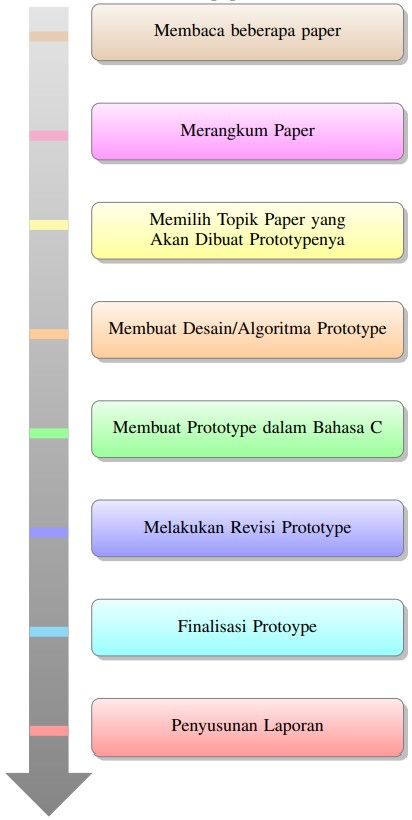
\includegraphics[scale=0.75]{pic1}
\end{figure}
\newpage
\section{impelementasi dan pengujian}

\subsection{Implementasi Graph pada Array dalam Bahasa C}

Program akan dimulai dengan pembacaan file bernama \textit {listtanaman.txt}. File tersebut akan menyimpan informasi men genai semua nama tanaman yang bersangkutan. Setelah pembacaan tersebut, akan dicari informasi mengenai bobot graph yang menghubungkan node. Informasi ini disimpan di dalam matriks segitiga bawah kiri didalam file \textit {jarakantarpohon.txt} yang juga dibuka saat program dijalankan. Matriks menggambarkan bobot antara jarak dua node tanaman sekali saja karena pemodelan \textit {undirected} graph yang memiliki jarak sama baik dari \textit a ke \textit b maupun \textit b ke \textit a. Nilai -1 akan menggambarkan bagian \textit {node} yang tidak terhubung sama sekali dalam graph dan juga dinyatakan dalam suatu variabel bernama int max (Jaraknya sebesar tak hingga). Nilai jarak terpendek akan disimpan dalam array tersebut selagi program berjalan.
\subsection{Implementasi Algoritma Djikstra dalam Bahasa C}
	Dalam implementasi algoritma, abstraksi dengan menggunakan pseudocode dapat dibagi menjadi dua buah fungsi dan satu program utama. Fungsi yang digunakan adalah fungsi printgraph (Fungsi Graph) untuk memunculkan graph berukuran $n \times n$ ke layar pengguna. Algoritma dari fungsi tersebut dapat dilihat pada bagian di bawah ini:
\begin{algorithm}
\caption{Fungsi Graph \ttfamily{(printgraph)}}\label{alg:two}
\KwResult{Memunculkan Graph $n \times n$ Ke Layar}
\textbf{procedure} \textit{printgraph(n, graph[n][n])}
\newline
\While{$i \leq n - 1$}{
	$j \gets 0$\;
	\While{$j \leq n-1$}{
		\eIf{$graph[i][j] = int\_max$}{
			\KwOut{-1;}
		}{
			\KwOut{$graph[i][j]$;}
		}
		$j \gets j + 1$\;
	}
	$i \gets i + 1$\;
}
\end{algorithm}
	
Fungsi kedua yang digunakan adalah fungsi pencari indeks pada array yang akan diproses dengan menggunakan pendekatan algoritma Dijkstra. Abstraksi fungsi yang digunakan dapat dilihat pada bagian berikut ini:
\begin{algorithm}
\caption{Fungsi Pencari Indeks \ttfamily{idx\_process}}\label{alg:three}
\KwResult{Mencari indeks yang akan diproses dengan algoritma Djikstra}
\textbf{Initialization:}

$is\_found \gets FALSE$\;
$i \gets 0$\;
\textbf{Algorithm:}

\While{$i \leq n-1$}{
	$j \gets 0$\;
	\If{!is\_final[i] \textbf{and} is\_found}{
		$idx\_min \gets i$\;
		$val\_minimum\gets jarak\_f[i]$\;
		$is_found\gets true$\;}

	\If{is\_found \textbf {and} is\_final[i] \textbf {and}  (jarak\_f[i] \textless val\_minimum)}{
		$idx\_min \gets i$\;
		$val\_minimum \gets jarak\_f[i]$\;}

}
\eIf{is\_found}{
	\Return{(idx\_min)}
}{
	\Return{(int\_max)}
}
\end{algorithm}

	Program utama akan membaca file database tanaman beserta jarak masing-masing tanaman dan akan mencetak daftar tanaman yang berada di Kebun Raya Purwodadi. Kemudian, program akan menerima input salah satu tanaman terdekat dari pengguna sebagai penanda posisi awal pengguna. Setelah itu, program akan kembali menerima input posisi tanaman tujuan dan memproses pencarian rute terdekat dengan algoritma Dijkstra. Rute yang diperlukan akan ditampilkan dalam bentuk list nama tanaman yang harus dilalui pengguna dan menampilkan jarak antara kedua tanaman tersebut. Implementasi algoritma dalam abstraksi tersebut dapat dilihat pada gambar di bawah ini:
\begin{algorithm}
\caption{Program Utama Pencarian Rute Antara Dua Tanaman - Pembacaan Jumlah Tanaman}\label{alg:four}
\KwResult{Menyimpan nama tanaman pada sebuah array}
\textbf{Algorithm:}

\textbf{input}($namafile\_tanaman$)\;
\textbf{open}($namafile\_tanaman$)\;
\textbf{read}($namafile\_tanaman$)\;
$n\_tanaman \gets 0$\;
$baris \gets 0$\;
\While{$baris \leq max\_len$}{
	$token \gets parse(baris)$\;
	$token \gets nama\_tanaman[n\_tanaman]$\;
	$baris \gets baris+1$\;
}
\end{algorithm}
	
	Setelah pembacaan jumlah tanaman dari file, maka diperlukan graph atau jarak antar tanaman yang akan menjadi dasar perhitungan dari pencarian rute terdekat. Proses memasukkan graph dapat dilihat pada algoritma berikut ini:
\begin{algorithm}
\caption{Program Utama Pencarian Rute Antara Dua Tanaman - Memasukkan Graph}\label{alg:five}
\KwResult{Menyimpan gray dalam sebuah matriks $n \times n$}
\textbf{input}($namafile\_graph$)\;
\textbf{open}($namafile\_graph$)\;
\textbf{read}($namafile\_graph$)\;
$baris \gets 0$\;
\While{$baris\leq max\_len$}{
	$k \gets 0$\;
	$token \gets parse(baris)$\;
	\While{$token! = NULL$}{
		$graph[j][k] \gets token$\;
		$graph[k][j] \gets token$\;
		\eIf{token == -1}{
			$graph[j][k] \gets int\_max$\;
			$graph[k][j] \gets int\_max$\;
		}{
			$k \gets k + 1$\;
			$token \gets parse(NULL)$\;
}
}
$baris \gets =baris + 1$\;
}
\end{algorithm}
\newpage
	Setelah data yang dibutuhkan dimasukkan, implementasi dari algoritma Dijkstra untuk pencarian rute terdekat adalah sebagai berikut:
\begin{algorithm}
\caption{Program Utama Pencarian Rute Antara Dua Tanaman: Pencarian Jarak dengan Algoritma Dijkstra}\label{alg:six}
\textbf{Algorithm:}

\textbf{input}($idx\_a$)\;
$idx\_a \gets idx\_a-1$\;
\textbf{input}($idx\_tujuan$)\;
$idx\_tujuan \gets idx\_tujuan-1$\;
\For{i= 0 \emph{\KwTo} n\_tanaman}{
	\eIf{$i = idx\_a$}{
		$jarak\_f[i] \gets 0$\;
		$is\_final[i] \gets FALSE$\;
	}{
		$jarak\_f[i] \gets int\_max$\;
		$is\_final[i] \gets FALSE$\;
}
	\For{j= 0 \emph{\KwTo} n\_tanaman}{
		$list\_dilalui[i][j] \gets int\_max$\;
}
		$idx\_lalui[i] \gets 0$\;
}
$jarak\_f[idx\_[a] \gets 0$\;
$list\_dilalui[idx\_a] [0] \gets idx_a$\;
$idx\_lalui[idx\_a] \gets idx\_lalui[idx\_a]+1$\;
$idx\_now \gets idx\_a$\;
\While{$idx\_now! = int\_max$}{
	$is\_final [idx\_now] \gets TRUE$\;
	\For{i= 0 \emph{\KwTo} n\_tanaman-1}{
		\If{(!is\_final[i] \textbf {and} graph[idx\_now][i] != int\_max  \textbf {and} (jarak\_f[idx\_now] + graph[idx\_now][i] > jarak\_f[i]}{
			$jarak\_f[i]) \gets (jarak\_f[idx\_now] + graph [idx\_now][i]$\;
			$idx\_lalui[i] \gets idx\_lalui [idx\_now] + 1$\;
			}
		\For{j= 0 \emph{\KwTo}  idx\_dilalui[i]-1}{
			\eIf{$j = idx\_dilalui[i]-1$}{
				$list\_dilalui[i][j] \gets i$\;
			}{
				$list\_dilalui[i][j] \gets list\_dilalui[idx\_now][j]$\;
			}
}
}
$idx\_now \gets idx\_process (n\_tanaman, jarak\_f, is\_final)$\;
}
\end{algorithm}
\newpage
\subsection{Perhitungan Kompleksitas Waktu}
	Kompleksitas dari program ini dengan notasi kompleksitas Big O adalah O($n^2$). Hal tersebut disebabkan pada loop program bagian for, terdapat loop for lain yang berjumlah dua loop (Terletak pada bagian assign kondisi awal dan ketika program menjalankan algoritma Djikstra). Karena hal tersebut, akibatnya adalah kompleksitas waktu akan naik seiring dengan naiknya n program yang dijalankan, namun tidak bersifat linear sehingga kompleksitas waktunya adalah O($n^2$). Grafik kompleksitas waktu dapat direpresentasikan pada gambar 1.
\begin{figure}[htbp]
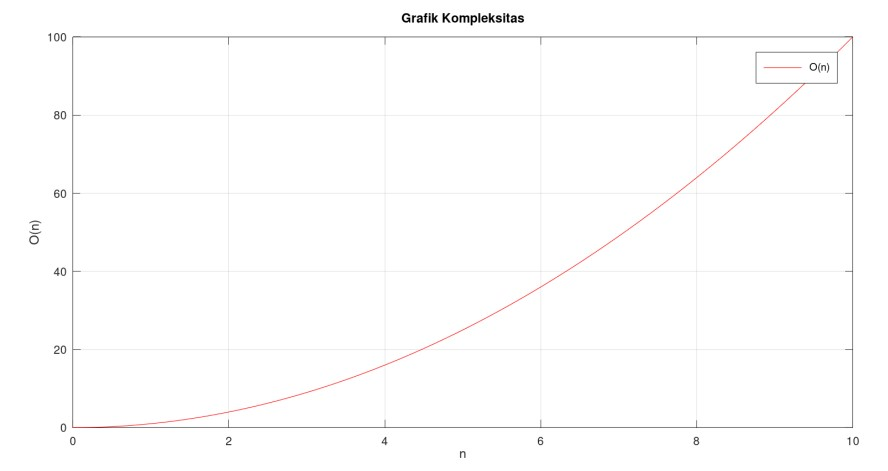
\includegraphics[scale=0.55]{pic2}
\caption{Kompleksitas Waktu Program}
\end{figure}
\subsection{Perhitumgan Kompleksitas Tempat}
	Matriks penyimpanan yang digunakan pada program ini memiliki ukuran terbesar n × n, dengan nilai n merepresen tasikan banyak tanaman dalam file listtanaman.txt. Program akan melalui grafik dan menyimpan nilai bobot antara node sebesar matriks di atas, mengakibatkan program dengan kom pleksitas O($n^2$ ). Hal ini dapat dilihat pada grafik kompleksitas tempat di gambar 2.
\begin{figure}[htbp]
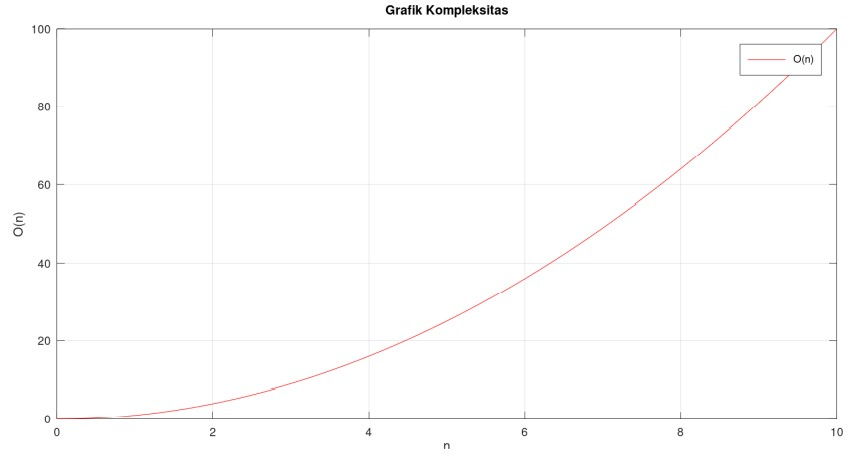
\includegraphics[scale=0.55]{pic3}
\caption{Kompleksitas Waktu Program}
\end{figure}
\section{kesimpulan}
	Pada perhitungan Jarak Terdekat dalam suatu lokasi atau ruang dapat diimplementasikan penggunaan Algoritma Djikstra dalam perhitungannya untuk mencapai suatu target pada ruang tersebut dari suatu titik. Terbukti dari penelitian Kebun Raya Purwodadi untuk menentukan Tanaman yang ingin dituju.
%Referensi
\bibliographystyle{IEEEtran}
\bibliography{references.bib}



\end{document}


